% !TEX encoding = UTF-8
% !TEX TS-program = pdflatex
% !TEX root = ../tesi.tex

%**************************************************************
\chapter{Conclusioni}
\label{cap:conclusioni}
%**************************************************************
\section{Consuntivo delle tempistiche}
\label{tempistiche}
Questo capitolo racchiude l'intero andamento del progetto di stage, passando per tutte le sue fasi.\\
La pianificazione oraria ha subito alcuni cambiamenti durante la durata dello stage. Questo perché mi è stato chiesto di dare maggiore priorità ad alcuni elementi ritenuti 
più importanti per l'azienda rispetto ad altri aspetti secondari che potevano essere colmati in altri modi. In particolare la parte di stesura di manuale utente e sviluppatore,
considerata opzionale, è stata tralasciata per dare maggior peso alla parte di test e validazione del prodotto. Inoltre si è scelto, assieme al tutor interno, di utilizzare
come appoggio i commenti a supporto del codice piuttosto che i manuali sopracitati. Anche la fase di stesura dell'analisi dei requisiti ha subito una variazione oraria, in quanto
l'aggiunta dei casi d'uso da me proposti ha ricevuto riscontri positivi ed è proseguita senza intoppi fin da subito.\\ Un lieve aumento lo si nota sulla fase di studio delle
tecnologie utilizzate, in quanto dovevo familiarizzare con strumenti che non avevo mai utilizzato, quali DevExpress e vb.NET, la loro padronanza ha richiesto più del dovuto.\\
Infine, come anticipato, la fase di test e validazione ha subito un aumento in quanto, l'accertamento della bontà della soluzione richiedeva un considerevole ammontare di tempo
sia da parte mia che da parte del tutor interno. Questo tempo ha inoltre incluso la fase di controllo statica del codice durante la stesura delle nuove unità e controlli dinamici
durante l'esecuzione dell'applicativo.
\newpage


\renewcommand{\arraystretch}{1.5}
\rowcolors{2}{dispari}{pari}
\arrayrulecolor{white}
\begin{longtable}{ >{\centering}p{0.15\textwidth} >{}p{0.60\textwidth}
    >{\raggedright}p{0.15\textwidth} >{\centering}p{0.14\textwidth}}
	\caption{Ore effettive}
	\label{effettive}
\\
\rowcolorhead 
\textbf{\color{white}Ore preventivate} 
& \textbf{\color{white}Descrizione} 
& \centering\textbf{\color{white}Ore effettive}
 

\endhead	

40	&	Analisi del modulo software esistente, funzionalità da realizzare e documentazione disponibile dell’algoritmo esistente	&	\centering 40	\tabularnewline
12	&	Analisi dei requisiti e stesura della relativa documentazione	&	\centering 4(-8)	\tabularnewline
16	&	Studio delle tecnologie aziendali necessarie allo sviluppo del modulo 	&	\centering 20(+4)	\tabularnewline
40	&	Studio di algoritmi e tecniche di Ricerca Operativa e Ottimizzazione Combinatoria	&	\centering 40 	\tabularnewline
128	&	Sviluppo delle componenti:
\begin{itemize}
    

\item Sviluppo procedura di gestione degli ordini fornitori
\item Sviluppo procedura di gestione delle giacenze di magazzino
\item Sviluppo procedura di gestione dei semilavorati pianificati
\item Integrazione dei vincoli del problema di ottimizzazione con i nuovi parametri
\item Algoritmo Greedy: sviluppo di nuove strategie di scelta del passo successivo adottato dall’algoritmo nella costruzione della soluzione del problema
\item Integrazione della Tabu Search con nuovi meccanismi: criteri di aspirazione e arresto, variazione dei meccanismi di esplorazione del vicinato e adozione di tecniche di intensificazione e diversificazione	
\end{itemize} &	\centering 132(+4) 	\tabularnewline
60	&	Validazione e test	&	\centering 80(+20) 	\tabularnewline
24	&	Stesura della documentazione del prodotto sviluppato	&	\centering 4(-20) 	\tabularnewline
\end{longtable}

\newpage
\section{Consuntivo dell'analisi dei rischi}

Si sono verificati due dei tre casi preventivati nella fase di analisi dei rischi.\\ Il primo riguarda il rischio \textit{RT1-Inesperienza tecnologica} con il quale mi sono
scontrato nelle prime fasi del progetto. Il secondo riguarda \textit{RT2-Scelte implementative} il quale ha richiesto maggior tempo di verifica durante la codifica.


\renewcommand{\arraystretch}{1.5}
\rowcolors{2}{dispari}{pari}
\arrayrulecolor{white}
\begin{longtable}{ >{\centering}p{0.45\textwidth} >{}p{0.45\textwidth}
    >{\raggedright}p{0.15\textwidth} >{\centering}p{0.14\textwidth}}
    \caption{Consuntivo dell'analisi dei rischi}
\\
\rowcolorhead 
\textbf{\color{white}Descrizione} 
& \textbf{\color{white}Soluzione} 
 

\endhead	

Le nuove tecnologie da utilizzare si sono verificate più complicate del previsto, causato anche dal fatto di dover ampliare un progetto già esistente
con diverse funzionalità avanzate già implementate &	Ho fatto uso della documentazione a supporto dell'applicativo e dell'aiuto del tutor interno che mi dava
indicazioni ad ogni passo di esecuzione dell'algoritmo		\tabularnewline
Le varie scelte implementative spesso conducevano a strade senza uscita, dalle quali era necessario ricominciare con una nuova progettazione del codice	&
Tramite l'aiuto del tutor interno e delle conoscenze ormai acquisite sono sempre riuscito a trovare tecniche alternative per portare al termine il progetto	\tabularnewline

\end{longtable}

\newpage
\section{Soddisfacimento dei requisiti e raggiungimento degli obiettivi}

Tutti i requisiti obbligatori sono stati soddisfatti, i quali formavano le fondamenta del progetto di stage ed erano considerati di fondamentale importanza per l'azienda.
Si è raggiunta la totalità dei requisiti desiderabili, i quali davano lustro alle funzionalità dell'applicativo e ne accrescevano l'insieme di funzionalità. I due requisiti
facoltativi non soddisfatti riguardano la stesura dei manuali, convertita in aggiunta di commenti durante la codifica.\\


\renewcommand{\arraystretch}{1.5}
\rowcolors{2}{dispari}{pari}
\arrayrulecolor{white}
\begin{longtable}{ 
		>{\centering}p{0.17\textwidth} 
		>{\raggedright}p{0.28\textwidth}
		>{\raggedright}p{0.29\textwidth} 
		>{\centering}p{0.15\textwidth}
	}
	
	\caption{Requisiti soddisfatti}\\
	\rowcolorhead
	\colorhead\textbf{Stato} & \centering\colorhead\textbf{Obbligatori} & 
	\centering\colorhead\textbf{Desiderabili} & 
	\colorhead\textbf{Facoltativi} 
	\tabularnewline
	\endfirsthead
	\rowcolor{white}\caption[]{(continua)}\\
	\rowcolorhead
	\colorhead\textbf{Stato} & \centering\colorhead\textbf{Obbligatori} & 
	\centering\colorhead\textbf{Desiderabili} & 
	\colorhead\textbf{Facoltativi} 
	\tabularnewline
	\endhead
	
	%RO1---------------------------------------------------------
	\rowcolordark  Soddisfatti & 
	\centering 24 &
	\centering 5 &
	\centering 0	
	\tabularnewline
	
	%RO2---------------------------------------------------------
	\rowcolorlight Non soddisfatti & 
	\centering \\0 &
	\centering \\0 &
	\centering \\2	
	\tabularnewline

	
\end{longtable}


Per quanto riguarda gli obiettivi opzionali ne è stato scartato uno in seguito ad un colloquio con il tutor aziendale, secondo il quale non valeva la pena di sovraccaricare il programma con dei
dati ridondati per eseguire una ripianificazione. Si è scelto quindi di pianificare partendo da zero con i nuovi dati. Di seguito sono riportati in grafico i requisiti e il loro
Soddisfacimento.\\ Gli altri obiettivi sono stati ampiamente raggiunti durante le rispettive fasi dello sviluppo dell'applicativo.

\begin{figure}[H]
	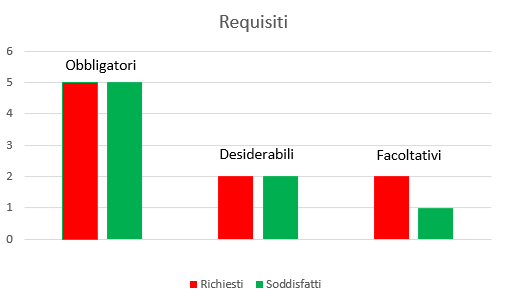
\includegraphics[width=13cm]{immagini/requisiti.png}
	\centering
	\caption{Obiettivi raggiunti}
\end{figure}


\section{Conoscenze acquisite}

Durante il percorso di stage ho acquisito nuove conoscenze sia in ambito tecnico che di sviluppo sottostando ad esigenze reali. 

\subsection{Vb.NET, DevExpress e Informix}

Sono le tecnologie che più ho utilizzato durante lo svolgimento dello stage, e mi sono servite durante tutto l'arco di codifica e testing.\\
Essendo la prima volta che mi interfacciavo con queste tecnologie ho riscontrato alcuni problemi in partenza, dovuti appunto all'inesperienza e al fatto che il mio 
progetto si integrava ad uno esistente. La base teorica comunque è riconducibile a qualsiasi altro linguaggio di programmazione visto anche in ambito universitario
per quanto riguarda Vb.NET. \\Per quanto riguarda Informix si sono rese sufficienti le conoscenze teoriche e pratiche conseguite durante il percorso di studi, si è resa
necessario qualche intervento da parte del tutor aziendale in casi particolari di formattazione delle tabelle che andavo ad utilizzare.\\
DevExpress ha avuto un ruolo marginale rispetto ai precedenti ma è comunque servito ad interpretare correttamente le funzionalità dell'interfaccia grafica sulla quale dovevo
apportare le modifiche richieste. Al termine dello stage posso affermare che ho acquisito la piena padronanza di queste tecnologie non solo a livello superficiale ma anche
andando più in profondità, altre conoscenze derivano dal fatto di prolungare il loro utilizzo in futuro.\\

\subsection{Metodo di lavoro}

È la prima volta che mi pongo dinanzi ad un progetto di tali dimensioni in solitaria, ciò mi ha permesso di imparare a gestire le varie scadenze e consegne entro dei limiti
imposti da un vero e proprio mondo del lavoro. \\Inizialmente ho leggermente sottovalutato le ore di studio del problema esistente, non per negligenza ma perché non mi è parso
chiaro sin da subito l'entità del problema che dovevo affrontare, fino a quando non ho effettivamente iniziato a lavorarci.\\ Ciò ha inizialmente rallentato la fase di sviluppo
in quanto dovevo porre frequenti domande al tutor anche per aiutarmi ad entrare nell'ottica della pianificazione eseguita sui generi alimentari di cui tratta l'azienda.\\ Ciò mi
ha concesso di capire quanto sia importante chiarire ogni dubbio prima di iniziare a lavorare sulla soluzione del problema, così da non causare un effetto cascata in seguito.
Nelle fasi successive, grazie a tale esperienza, non ho avuto problemi al di fuori di questioni legate a vincoli reali di pianificazione ed è stato possibile proseguire senza
rallentamenti.

\subsection{Scadenze}

Anche in questo caso ho dovuto riadattare il mio regime di lavoro in base alle scadenze imposte.\\ Avendo già avuto a che fare con problemi di \hyperref[Scheduling]{scheduling\glo} del lavoro,
mi sono affidato ad un calendario che ho compilato dal primo giorno di stage, nel quale inserivo i vari obiettivi da raggiungere settimanalmente e giornalmente. Con questo
sono riuscito a garantire un ottimo flusso di esecuzione delle operazioni da portare al termine in modo lineare ed efficacie. Nel caso di problematiche esterne ho valutato dei
possibili tempi di stallo nel \hyperref[Planning]{planning\glo} così da avere un margine di scarto in ogni settimana lavorativa.

\section{Università e mondo del lavoro}

Ho sempre avuto la tendenza a valutare il mondo scolastico completamente separato dal mondo del lavoro. Questo perché alcune conoscenze tendono a fermarsi al livello teorico
senza però scendere nel dettaglio e quindi mancanti della parte pratica. Al contrario nel mondo del lavoro ho sempre pensato che sia la pratica a far da padrone e che quindi
risultasse sì utile il grado di preparazione teorica, ma che non avesse la stessa rilevanza in termini di capacità richieste ad un qualsiasi lavoratore. Dopo questo stage posso
invece affermare che il grado di conoscenza teorico è di gran lunga superiore al grado di conoscenza pratico ed è un elemento fondamentale che un qualsiasi buon programmatore 
deve avere.\\ Durante il progetto ho dovuto spaziare tra diversi campi che vanno dall'Ingegneria del Software alla Ricerca Operativa, passando per altre decine di conoscenze
che se non avessi frequentato l'Università non avrei padroneggiato. Inoltre ho valutato importantissima la capacità di saper imparare nuovi concetti e acquisire informazioni,
grazie al metodo di studio affinato durante il percorso di studi, la quale supera di gran lunga la capacità di saper semplicemente utilizzare un qualsiasi strumento
di sviluppo o simili.\\ In sostanza sono fermamente convinto che anche un percorso di studi triennale fornisca le competenze necessarie e sufficienti per approcciarsi in modo
corretto al mondo del lavoro.

\subsection{Valutazione personale}

L'intero progetto di stage è stato svolto sotto la supervisione del tutor aziendale che però non ha partecipato attivamente allo sviluppo del progetto, anzi ha cercato di 
lasciarmi quanto più spazio possibile cosicché possa trovare da solo una soluzione ai problemi che, molto probabilmente, dovrò riaffrontare in futuro. Ovviamente era sempre
disponibile in caso di problematiche che andassero al dì la della mia comprensione in materia di politiche aziendali e anche nel caso in cui dovessi affrontare dei problemi
implementativi di spessore.\\ Il fatto di doversi gestire con le tempistiche e le varie scadenze ha accresciuto molto la mia competenza di giudizio sulle mie reali capacità.
Inoltre il rapporto coi colleghi mi ha aiutato ad entrare, soprattutto mentalmente, nell'ideologia lavorativa condivisa in azienda e anche questo mi ha permesso di crescere
a livello personale.\\ In conclusione ritengo il periodo di stage un fattore di crescita personale di fondamentale importanza per uno studente universitario. Ti permette di capire
se il tuo percorso di studi è stato utile e se effettivamente è il lavoro che intendi fare una volta concluso il proprio percorso.\\ Lo ritengo fondamentale in un corso di studi
come il nostro e sono d'accordo che sia obbligatorio per conseguire il titolo di studio.